\documentclass[letterpaper]{article}
\usepackage[submission]{aaai2027}

\usepackage{graphicx}
\usepackage{natbib}
\usepackage{caption}
\usepackage{algorithm}
\usepackage{algorithmic}
\usepackage{booktabs}
\usepackage{tabularx}
\usepackage{amsmath}
\usepackage{float}
\title{Supplementary Material for SPEM: Structure-Aware Procedural Memory for Efficient Skill Use in LLM Agents}

\newcommand{\model}{\textsc{SPEM}}
%

\setcounter{secnumdepth}{3}


\begin{document}
\maketitle
\appendix
\setcounter{section}{0}
\setcounter{subsection}{0}
\setcounter{subsubsection}{0}

% Put these AFTER \appendix, otherwise \appendix may overwrite them.
\renewcommand{\thesection}{\Alph{section}}
\renewcommand{\thesubsection}{\Alph{section}.\arabic{subsection}}
\renewcommand{\thesubsubsection}{\Alph{section}.\arabic{subsection}.\arabic{subsubsection}}


\begin{abstract}
This supplementary material provides additional implementation details,
experimental results, sensitivity analyses, and case studies for the main paper.
\end{abstract}

\section{Method Details}
\subsection{Overall Inference Protocol}
\label{app:overall_inference}

Algorithm~\ref{alg:overall_inference} summarizes the inference protocol of
\model{}. Given a task request and the current execution state, the system first
retrieves relevant atomic skills and previously extracted Skill-DAG templates.
If a confident template is matched, \model{} injects it as structured procedural
guidance. Otherwise, it falls back to a bounded set of retrieved atomic skills.
During execution, Skill-GNN can be invoked on demand to rerank candidate skills
under the current task, state, and execution history. After the episode
terminates, successful trajectories are converted into Skill-DAG templates and
written back to memory, while failed executions only update reliability
statistics for the used skills or templates.


\begin{algorithm}[h]
\caption{Overall Inference of \model{}}
\label{alg:overall_inference}
\begin{algorithmic}[1]
\REQUIRE task request $q$, initial state $s_0$, Atomic Skill Memory $\mathcal{M}_a$, Skill-DAG Memory $\mathcal{M}_d$
\ENSURE execution result and updated memory

\STATE Retrieve atomic candidates $\mathcal{C}_a$ from $\mathcal{M}_a$
\STATE Retrieve Skill-DAG templates $\mathcal{C}_d$ from $\mathcal{M}_d$

\IF{a confident template exists in $\mathcal{C}_d$}
    \STATE Inject the best Skill-DAG template as procedural guidance
\ELSE
    \STATE Inject top atomic candidates from $\mathcal{C}_a$
\ENDIF

\STATE Initialize trajectory $\tau \leftarrow \emptyset$ and state $s \leftarrow s_0$

\WHILE{the task is not terminated}
    \IF{replanning is triggered}
        \STATE Construct a task-conditioned candidate graph $G(q,s,\tau)$
        \STATE Rerank candidate skills with Skill-GNN
        \STATE Inject top-ranked skills as state-aware guidance
    \ENDIF
    \STATE Agent executes the next action under current guidance
    \STATE Observe new state $s'$ and append the transition to $\tau$
    \STATE $s \leftarrow s'$
\ENDWHILE

\IF{the task succeeds}
    \STATE Extract a Skill-DAG $G_\tau$ from $\tau$
    \STATE Insert or reinforce $G_\tau$ in $\mathcal{M}_d$
\ELSE
    \STATE Update reliability statistics of used skills/templates
\ENDIF
\STATE \RETURN execution result
\end{algorithmic}
\end{algorithm}


\subsection{Memory Schemas}
\label{app:memory_schemas}

\model{} maintains two complementary memory stores: Atomic Skill Memory and
Skill-DAG Memory. Table~\ref{tab:memory-schema} summarizes the main fields and
their roles. Atomic Skill Memory stores individual reusable capabilities, while
Skill-DAG Memory stores procedural templates extracted from successful
executions.

For Atomic Skill Memory, each atomic skill contains three categories of
information. The first category consists of static identity and semantic fields,
which describe what the skill is designed to do. These fields include a stable
identifier, skill name, source path, version, natural-language description, and
a short task-facing capability summary. In our implementation, the retrieval
embedding is computed from the skill name and the one-line capability summary,
so first-stage retrieval focuses on matching the current task to the skill's
task-facing functionality; the full skill document is preserved for prompt
construction after retrieval. The second category consists of interface fields,
which describe how the skill can be invoked, including input and output schemas,
software or tool dependencies, and device or environment requirements. These
fields help the agent use the skill correctly and provide structured signals
for candidate graph construction and compatibility reasoning between neighboring
skills. The third category consists of lightweight dynamic statistics collected
during online use, including usage count, empirical success rate, execution
cost, last-used timestamp, and user preference score. These statistics are
updated after execution and can be used for reranking or personalization. They
are conservatively initialized and updated with an exponential moving average,
allowing the memory to adapt to deployment feedback without changing the
underlying skill definition.

A Skill-DAG is a directed acyclic graph whose nodes correspond to mapped atomic
skills or abstract procedural phases, and whose edges encode typed dependencies
such as temporal, data-flow, control-flow, and argument dependencies. Each
Skill-DAG also stores the source task description, a task embedding for template
retrieval, provenance metadata, dynamic reliability statistics, and a structural
signature for deduplication and merging. During inference, atomic skills and
Skill-DAG templates are retrieved by cosine similarity in their respective
embedding spaces. After execution, only successful trajectories can insert new
Skill-DAG templates; failed executions update reliability statistics but do not
create positive procedural memory.

\begin{table*}[t]
\centering
\small
\begin{tabularx}{\textwidth}{>{\centering\arraybackslash}p{0.10\textwidth} p{0.12\textwidth} p{0.34\textwidth} X}
\toprule
Memory & Sub-type & Key Fields & Purpose \\
\midrule
\multirow{Atomic Skill} & Core & \texttt{skill\_id}\newline\texttt{name}\newline\texttt{one\_line\_capability}\newline\texttt{description}\newline\texttt{semantic\_embedding} & Represent individual reusable capabilities and support task-skill retrieval. \\
\cmidrule{2-4}
 & Interface & \texttt{input\_schema}\newline\texttt{output\_schema}\newline\texttt{tooling}\newline\texttt{device\_requirements}\newline\texttt{raw\_content} & Describe how a skill can be invoked and provide full skill content for prompt injection. \\
\cmidrule{2-4}
 & Statistics & \texttt{success\_rate}\newline\texttt{exec\_cost}\newline\texttt{usage\_count}\newline\texttt{last\_used\_at} & Track online reliability and cost for reranking or adaptation. \\
\midrule
\multirow{DAG} & Template & \texttt{dag\_id}\newline\texttt{task\_description}\newline\texttt{task\_embedding}\newline\texttt{nodes}\newline\texttt{edges} & Store reusable multi-step procedural structures extracted from successful executions. \\
\cmidrule{2-4}
 & Node/Edge & \texttt{skill\_id}\newline\texttt{action\_type}\newline\texttt{arg\_tokens}\newline\texttt{edge\_type}\newline\texttt{dep\_source}\newline\texttt{weight} & Represent skill bindings, procedural phases, and typed dependencies between steps. \\
\cmidrule{2-4}
 & Metadata & \texttt{meta}\newline\texttt{structural\_signature}\newline\texttt{success\_rate}\newline\texttt{usage\_count}\newline\texttt{parent\_dag\_ids} & Support provenance tracking, deduplication, merging, and reliability-aware reuse. \\
\bottomrule
\end{tabularx}
\caption{Compact schema of the two memory stores used by \model{}.}
\label{tab:memory-schema}
\end{table*}


\subsection{Trajectory-DAG Extraction}
\label{app:trajectory_dag_extraction}

Trajectory-DAG extraction converts successful executions into reusable
procedural templates. It complements the memory update step in
Algorithm~\ref{alg:overall_inference} by specifying how an interaction trace is
compressed into a Skill-DAG. We first normalize environment-specific logs into
an ordered trajectory
\[
\tau=\{(a_t,o_t,r_t,y_t,b_t)\}_{t=1}^{T},
\]
where $a_t$ and $o_t$ denote the action and observation, $r_t$ and $y_t$ are
optional reward and completion signals, and $b_t$ is an optional runtime skill
binding.

For each normalized step, the extractor parses the action into a lightweight
schema containing the operation verb, argument spans, and mentioned entities.
It then builds an intermediate execution graph with step nodes and typed
dependencies: temporal edges connect adjacent useful steps, entity-dependency
edges connect steps sharing task-relevant entities or arguments, and terminal
edges connect completion-related steps to the success node.

To avoid storing noisy exploration, the extractor keeps only a compact execution
backbone. It seeds the retained set with terminal or positive-reward steps and
scans the trajectory backward to preserve prerequisite steps that introduce
required entities, satisfy argument dependencies, or directly support retained
steps. Low-information no-op steps, explicit failures, and redundant exploration
are removed. In implementation, each step receives an interpretable usefulness
score:
\[
u_t=\mathrm{clip}_{[0,1]}(\mathbf{w}^{+}\cdot\phi^{+}(t)
-\mathbf{w}^{-}\cdot\phi^{-}(t)),
\]
where $\phi^{+}$ includes progress, success, novelty, and dependency-support
signals, and $\phi^{-}$ includes failure, no-op, and redundancy signals. The
score is used only for pruning and diagnostics, not as verifier supervision.

Finally, contiguous retained steps with the same procedural intent are merged
into phase-level DAG nodes. Each node stores the inferred operation type,
task-relevant entities, compact supporting evidence, and optional skill
bindings. Retained dependencies are mapped into temporal, data-flow, or
control-flow edges; if no explicit dependency remains, the extractor falls back
to a temporal chain to preserve executability.

The extracted DAG is then used to update Skill-DAG Memory. Successful
executions insert new templates or reinforce matched ones, while successful
online replanning stores the revised trajectory as a new variant and lowers the
reliability of the original template. Failed executions do not create new
Skill-DAG templates and only update reliability statistics, preventing noisy or
unsuccessful behavior from being used as positive procedural memory.
\subsection{Cold-Start Deployment}

\model{} is designed to support both trajectory-rich and trajectory-scarce
deployment settings. The central question in cold-start deployment is whether
target-domain execution trajectories are available for training a
domain-specific Skill-GNN. If such trajectories are available, \model{}
constructs online-like graph training samples from trajectory prefixes and
trains an inductive Skill-GNN. If no target-domain trajectory is available,
\model{} performs a library-level warm start using only skill metadata to
construct pseudo task--skill pairs and weak skill--skill relations. During early
deployment, Atomic Skill Memory and available Skill-DAG templates provide the
primary guidance, while the warm-started Skill-GNN is used for bounded reranking.
Successful executions collected during deployment are then converted into
Skill-DAGs and transitions, which provide supervision for later Skill-GNN
adaptation.

A key reason why this transition is feasible is that Skill-GNN is inductive rather than transductive. It does not learn node embeddings tied to a fixed global skill graph. Instead, for each task state, \model{} dynamically constructs a candidate graph from retrieved atomic skills, task embeddings, state features, history features, and relation signals. Skill nodes are represented by semantic embeddings and execution-derived features, while message-passing parameters are shared across candidate graphs and edge types. Therefore, the trained Skill-GNN can be applied to unseen tasks, unseen candidate skill combinations, and newly extracted Skill-DAG variants as long as their features and relations can be constructed. This inductive design makes few-trajectory adaptation more practical in target domains.

In the trajectory-rich setting, each online-like sample is built from a prefix of a successful trajectory. The next skill is used as the target label, previous skills provide execution history, and a bounded candidate set is formed by combining the target skill, prefix-context skills, limited future positive skills, hard negatives retrieved from Atomic Skill Memory, and random negatives. The resulting graph contains task, state, history, and candidate skill features, but does not expose the full future DAG as model input. This prevents the model from relying on information unavailable during deployment.

In the trajectory-scarce setting, \model{} starts from a library-level warm
start rather than a trajectory-supervised graph model. Skill metadata are used
to build pseudo task--skill pairs and weak skill--skill relations, which provide
a lightweight initial structure for Skill-GNN. During early deployment, the
agent still relies primarily on Atomic Skill Memory retrieval and available
Skill-DAG templates, while the warm-started Skill-GNN is used only for bounded
reranking over retrieved candidates. As successful executions accumulate,
trajectory-DAG extraction converts them into reusable Skill-DAG templates and
training transitions, gradually adapting the system from retrieval-guided
cold start to structure-aware selection. Failed template executions are not
stored as new templates; they only reduce the reliability statistics of the
corresponding templates.

\subsection{Skill-GNN Training and Inference}
\begin{figure*}[t]
\centering
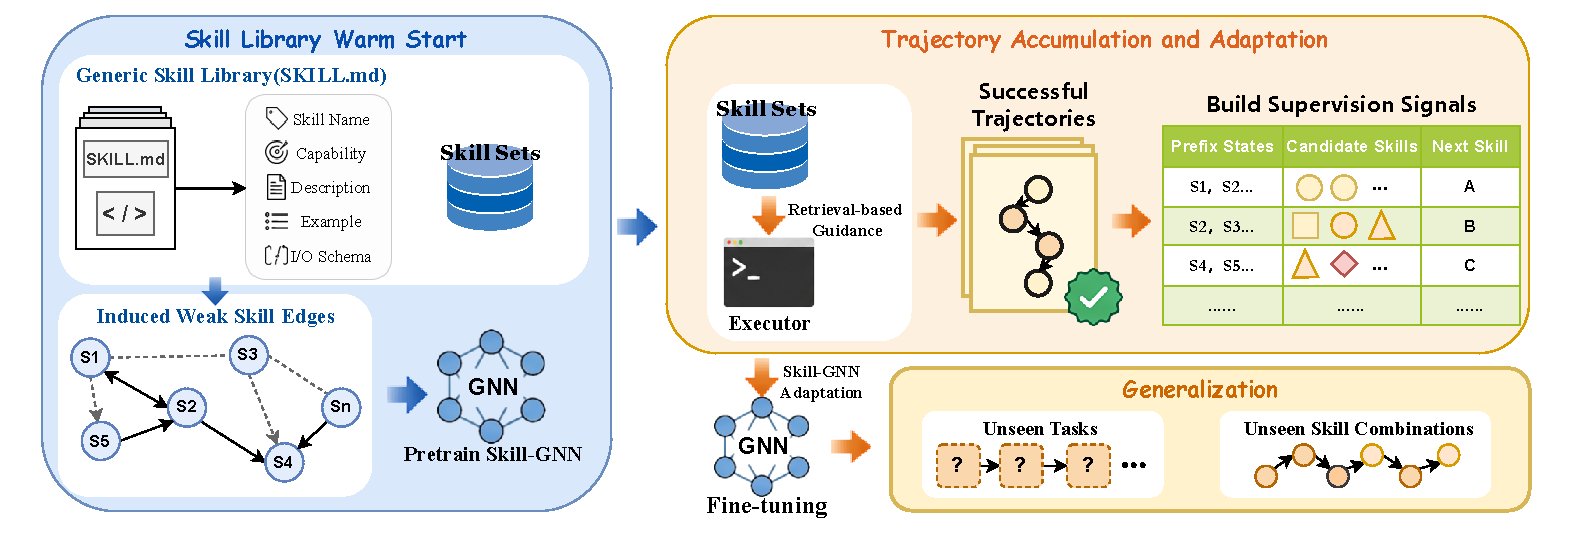
\includegraphics[width=\linewidth]{Figures/cold-start.pdf}
\caption{Cold-start deployment of \model{}. When no target-domain trajectories
are available, \model{} first warm-starts Skill-GNN from the generic skill
library by constructing pseudo queries and weak skill relations from skill
metadata. As successful executions accumulate, trajectories are converted into
prefix-level supervision signals for further Skill-GNN adaptation, enabling
generalization to unseen tasks and unseen skill combinations.}
\label{fig:cold_start}
\end{figure*}
\label{app:skillgnn_training}

\paragraph{Candidate graph construction.}
Skill-GNN is applied to a task-conditioned candidate graph rather than to a
fixed global skill graph. Given a task query, the system first retrieves a
bounded candidate set from Atomic Skill Memory. The graph contains a task node,
optional state and history nodes, and one node for each candidate skill. Node
features concatenate the corresponding semantic embedding with lightweight
dynamic statistics, including empirical success rate, preference score, usage
count, and execution cost. The graph contains typed edges from the task/state
context to candidate skills, as well as skill-skill edges induced by semantic
relatedness or template dependencies when available. This construction makes
Skill-GNN inductive: new tasks and newly added skills can be handled by building
a fresh candidate graph at inference time.

\paragraph{Prediction heads.}
Skill-GNN encodes the candidate graph and produces both node-level and
graph-level representations. We use three lightweight heads on top of the GNN.
The next-skill head scores candidate skill nodes conditioned on the current
selected prefix, the value head predicts the utility of the candidate graph, and
the edge head predicts whether two skill nodes should be connected by a
dependency edge. During online inference, the next-skill scores are used to
rerank candidate atomic skills before injecting them into the agent context.

\paragraph{Trajectory-supervised training.}
When successful trajectories are available, we train Skill-GNN with
trajectory-prefix supervision. For a successful Skill-DAG with ordered nodes
$(v_1,\ldots,v_m)$, each prefix $(v_1,\ldots,v_{k-1})$ defines a training state,
and the next node $v_k$ is used as the target skill. The next-skill objective is
a cross-entropy loss over candidate skill nodes:
\[
\mathcal{L}_{\mathrm{next}}
=
-\log
\frac{\exp f_\theta(v_k \mid G, P_k)}
{\sum_{v \in \mathcal{C}}\exp f_\theta(v \mid G, P_k)},
\]
where $P_k$ is the selected prefix and $\mathcal{C}$ is the candidate skill set.
When available, we additionally use a value loss for graph-level success or
reward prediction and a binary edge loss for dependency prediction:
\[
\mathcal{L}
=
\lambda_{\mathrm{next}}\mathcal{L}_{\mathrm{next}}
+
\lambda_{\mathrm{value}}\mathcal{L}_{\mathrm{value}}
+
\lambda_{\mathrm{edge}}\mathcal{L}_{\mathrm{edge}}.
\]
In our implementation, $\mathcal{L}_{\mathrm{value}}$ is a smooth-$L_1$ loss and
$\mathcal{L}_{\mathrm{edge}}$ is a binary cross-entropy loss over candidate node
pairs.

\paragraph{Library-level cold-start pretraining.}
Figure~\ref{fig:cold_start} shows the cold-start path used when no
target-domain trajectory is available. Starting from a generic skill library,
\model{} constructs pseudo queries from each skill's name, one-line capability,
description, example tasks, tooling, and I/O schema. The corresponding skill is
used as the positive target, while semantically or lexically similar skills are
sampled as hard negatives. In parallel, weak skill-skill edges are induced from
library metadata, including semantic neighbors, shared artifacts, shared tools
or tags, and compatible input-output schemas. These pseudo queries and weak
edges provide initial next-skill and edge supervision for Skill-GNN before any
successful task trajectory has been collected.

\paragraph{Leakage prevention.}
The training sources are separated according to the deployment setting.
Library-level pretraining uses only skill metadata and does not use task
solutions, verifier rewards, or evaluation trajectories. Trajectory-supervised
training uses only trajectories from the training split or successful
post-deployment executions. In particular, diagnostic query--gold pairs used for
retrieval analysis are not used to train the model. This prevents evaluation
tasks from being converted into positive supervision before they are executed.
\begin{table*}[t]
\centering
\small
\begin{tabular}{lcccccc}
\toprule
Backbone & Val Acc@1 & Test Acc@1 & Top-3 & MRR & Edge-F1 & Inference ms \\
\midrule
GAT &
$0.9676{\pm}0.0042$ &
$0.9776{\pm}0.0018$ &
$0.9991{\pm}0.0010$ &
$0.9878{\pm}0.0007$ &
$0.9741{\pm}0.0027$ &
$4.57{\pm}0.23$ \\
GIN &
$\mathbf{0.9728{\pm}0.0007}$ &
$\mathbf{0.9808{\pm}0.0008}$ &
$0.9994{\pm}0.0004$ &
$\mathbf{0.9901{\pm}0.0006}$ &
$0.9771{\pm}0.0025$ &
$\mathbf{1.47{\pm}0.04}$ \\
Hetero-GNN &
$0.9683{\pm}0.0004$ &
$0.9783{\pm}0.0030$ &
$\mathbf{0.9995{\pm}0.0012}$ &
$0.9885{\pm}0.0017$ &
$\mathbf{0.9841{\pm}0.0009}$ &
$2.42{\pm}0.71$ \\
\bottomrule
\end{tabular}
\caption{Skill-GNN backbone comparison. Runtime is measured as milliseconds per inference sample.}
\label{tab:gnn-backbone}
\end{table*}



\begin{table*}[t]
\centering
\small
\begin{tabular}{llccccc}
\toprule
Study & Setting & Test Acc@1 & Top-3 & MRR & Edge-F1 & Inference ms \\
\midrule
Candidate Top-$K$ & $K=8$  & $0.9533{\pm}0.0016$ & $0.9698{\pm}0.0004$ & $0.9613{\pm}0.0008$ & $0.9553{\pm}0.0011$ & $3.82{\pm}2.06$ \\
Candidate Top-$K$ & $K=16$ & $0.9490{\pm}0.0029$ & $\mathbf{0.9960{\pm}0.0012}$ & $0.9588{\pm}0.0016$ & $0.9546{\pm}0.0009$ & $3.81{\pm}0.75$ \\
Candidate Top-$K$ & $K=24$ & $0.9467{\pm}0.0084$ & $0.9693{\pm}0.0007$ & $0.9576{\pm}0.0044$ & $0.9582{\pm}0.0018$ & $3.31{\pm}0.77$ \\
Candidate Top-$K$ & $K=32$ & $\mathbf{0.9546{\pm}0.0021}$ & $\mathbf{0.9970{\pm}0.0008}$ & $\mathbf{0.9621{\pm}0.0011}$ & $\mathbf{0.9591{\pm}0.0014}$ & $\mathbf{2.58{\pm}0.21}$ \\
\midrule
Layers & 1 & $\mathbf{0.9520{\pm}0.0014}$ & $0.9695{\pm}0.0008$ & $\mathbf{0.9605{\pm}0.0012}$ & $0.9537{\pm}0.0029$ & $\mathbf{1.74{\pm}0.04}$ \\
Layers & 2 & $0.9490{\pm}0.0029$ & $\mathbf{0.9955{\pm}0.0010}$ & $0.9588{\pm}0.0016$ & $\mathbf{0.9546{\pm}0.0009}$ & $2.13{\pm}0.09$ \\
Layers & 3 & $0.9518{\pm}0.0026$ & $0.9695{\pm}0.0004$ & $0.9602{\pm}0.0016$ & $0.9503{\pm}0.0011$ & $2.73{\pm}0.06$ \\
\midrule
Hidden Dim & 64  & $\mathbf{0.9493{\pm}0.0044}$ & $0.9693{\pm}0.0007$ & $\mathbf{0.9589{\pm}0.0022}$ & $0.9519{\pm}0.0010$ & $\mathbf{2.12{\pm}0.08}$ \\
Hidden Dim & 128 & $0.9490{\pm}0.0029$ & $\mathbf{0.9965{\pm}0.0009}$ & $0.9588{\pm}0.0016$ & $\mathbf{0.9546{\pm}0.0009}$ & $2.16{\pm}0.05$ \\
Hidden Dim & 256 & $0.9483{\pm}0.0056$ & $0.9698{\pm}0.0004$ & $0.9588{\pm}0.0028$ & $0.9497{\pm}0.0052$ & $2.53{\pm}0.11$ \\
\midrule
Edge Neg. Ratio & 1 & $\mathbf{0.9520{\pm}0.0016}$ & $0.9698{\pm}0.0004$ & $\mathbf{0.9605{\pm}0.0007}$ & $\mathbf{0.9625{\pm}0.0009}$ & $2.62{\pm}0.32$ \\
Edge Neg. Ratio & 3 & $0.9490{\pm}0.0029$ & $\mathbf{0.9960{\pm}0.0010}$ & $0.9588{\pm}0.0016$ & $0.9546{\pm}0.0009$ & $\mathbf{2.45{\pm}0.19}$ \\
Edge Neg. Ratio & 5 & $0.9514{\pm}0.0010$ & $\mathbf{0.9970{\pm}0.0008}$ & $0.9601{\pm}0.0005$ & $0.9457{\pm}0.0046$ & $3.20{\pm}0.72$ \\
\bottomrule
\end{tabular}
\caption{Skill-GNN hyperparameter sensitivity. Results show that performance remains stable across candidate size, depth, hidden dimension, and edge negative sampling ratio.}
\label{tab:gnn-hyperparams}
\end{table*}



\begin{figure*}[t]
\centering
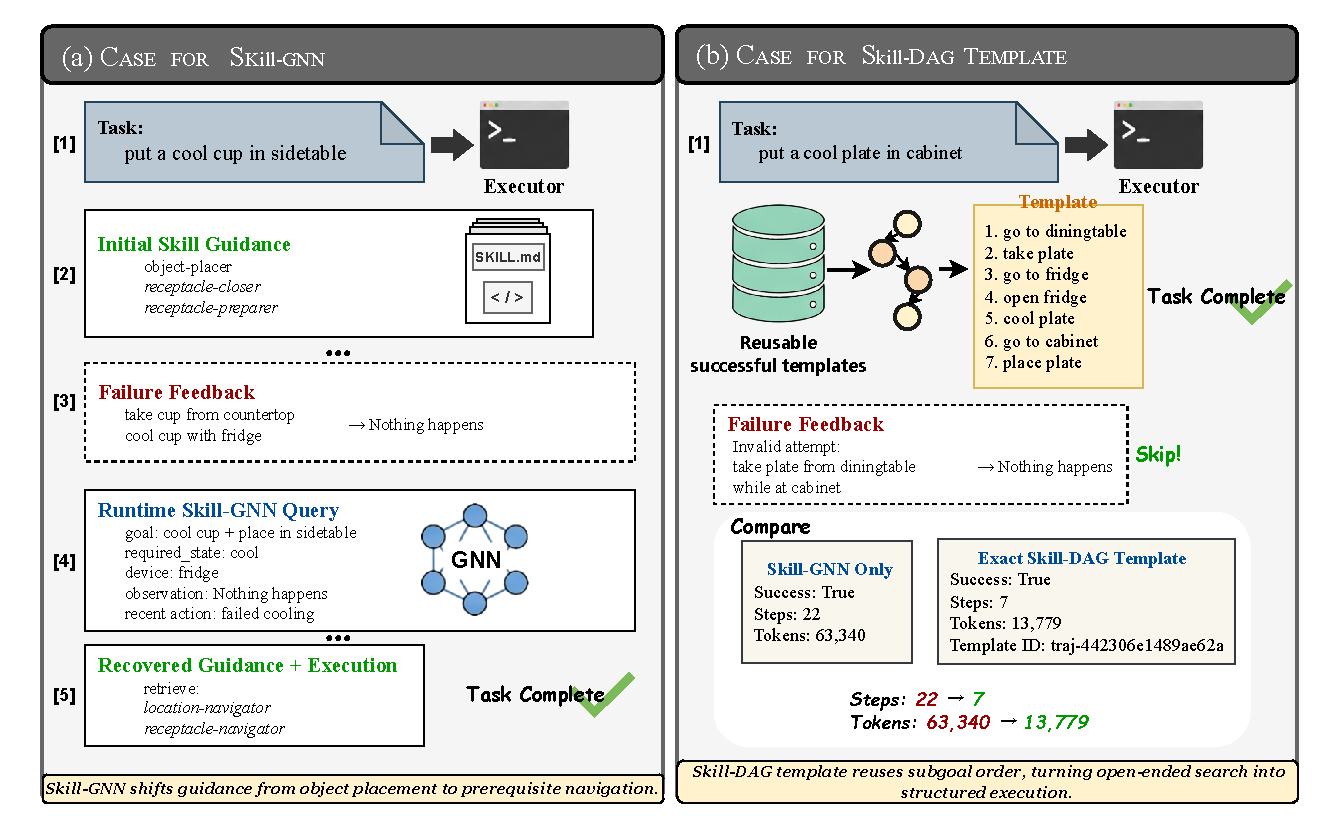
\includegraphics[width=\textwidth]{Figures/Case.pdf}
\caption{ALFWorld case studies illustrating the complementary roles of
Skill-GNN and Skill-DAG templates. As shown in (a), Skill-GNN provides
state-conditioned recovery guidance after a failed action by shifting the
agent's attention from object placement to prerequisite navigation. As shown in
(b), a retrieved Skill-DAG template reuses a compact successful subgoal order,
reducing redundant exploration and lowering both steps and token usage.}
\label{fig:case_studies}
\end{figure*}


\section{Experimental Details}
\label{app:experimental_details}

\paragraph{Fairness protocol.}
Across methods, we keep the benchmark split, skill library, agent interface,
execution environment, verifier, and evaluation script fixed whenever
applicable. Differences between methods are restricted to how skills are
selected, structured, and injected into the agent context. Offline memory
construction and Skill-GNN training are performed before evaluation and are not
counted as online execution time.

\paragraph{ALFWorld configuration.}
For ALFWorld, all skill-based methods use the same 37-skill library.
Atomic Skill Memory is constructed directly from the corresponding skill
documents. Skill-DAG Memory is constructed only from successful trajectories
outside the evaluation episodes. Skill-GNN is trained with trajectory-prefix
supervision: for each successful trajectory, a prefix of executed skills defines
the current procedural state, and the next executed skill is used as the
prediction target. The GNN is evaluated on disjoint development episodes and
does not access evaluation trajectories during memory construction or training.
The maximum number of environment interaction steps is set to 30.

\paragraph{SkillsBench configuration.}
For SkillsBench, all compared skill-based methods use the same
\texttt{skills\_200} library and the same Harbor-based agent execution
interface. Each task is allowed at most two attempts, with two concurrent trials,
following the GoS execution setting. Atomic Skill Memory is constructed from
skill names, capability summaries, descriptions, metadata, examples, and
interface schemas. Because target-domain successful trajectories may be
unavailable before evaluation, \model{} uses the library-level cold-start
procedure described above. Specifically, pseudo task--skill pairs are
constructed from skill metadata, and weak skill--skill edges are induced from
semantic similarity, shared tools or artifacts, tags, and schema compatibility.
When successful executions are later accumulated, their extracted Skill-DAGs can
be used for further Skill-GNN adaptation.

\paragraph{Key implementation parameters.}
Table~\ref{tab:key_impl_params} reports the main Skill-GNN implementation
parameters used in the trajectory-supervised setting. In ALFWorld, Skill-GNN is
trained from successful non-evaluation trajectories with trajectory-prefix
supervision. In SkillsBench, target-domain trajectories are scarce before
evaluation, so \model{} uses a library-level warm start constructed only from
skill metadata, pseudo task--skill pairs, and weak skill--skill relations. When
a small number of successful deployment trajectories become available, they can
be used for further adaptation, but evaluation-task trajectories are never used
for training. All runtime parameters are fixed within each benchmark and are not
tuned for individual tasks.

\begin{table}[t]
\centering
\small
\setlength{\tabcolsep}{5pt}
\renewcommand{\arraystretch}{1.08}
\begin{tabular}{ll}
\toprule
Parameter & Value \\
\midrule
GNN backbone & Hetero-GNN \\
Hidden dimension & 128 \\
GNN layers & 2 \\
Optimizer & AdamW \\
Learning rate & $1\times10^{-3}$ \\
Weight decay & $1\times10^{-5}$ \\
Batch size & 64 \\
Epochs & 5 \\
Template threshold & 0.80 \\
Decoding temperature & Benchmark default \\
\bottomrule
\end{tabular}
\caption{Key Skill-GNN implementation parameters in the trajectory-supervised
setting.}
\label{tab:key_impl_params}
\end{table}


\paragraph{Token and runtime accounting.}
For ALFWorld, token usage and runtime are averaged over evaluated episodes.
For SkillsBench, $T$ denotes raw input tokens rather than discounted
cached-token cost. $S$ measures only the agent execution phase. It includes
online skill retrieval, Skill-GNN reranking, and prompt construction when they
are invoked during agent execution, but excludes Docker image build time,
environment setup, dependency installation, and verifier runtime.

\paragraph{Leakage prevention.}
Library-level warm start uses only skill metadata and does not use task
solutions, verifier rewards, or evaluation trajectories. Trajectory-supervised
Skill-GNN training uses only training trajectories or successful
post-deployment executions. Diagnostic query--gold pairs used for retrieval
analysis are used only for analysis and are not used to train the model. Failed
executions do not create positive Skill-DAG templates and only update reliability
statistics.

\section{Additional Results}

\label{app:additional_results}

\subsection{Skill-GNN Backbone Comparison}
\label{app:gnn_backbone}

Table~\ref{tab:gnn-backbone} compares different GNN backbones in an offline
next-skill prediction setting. This diagnostic evaluates whether the model can
rank the correct next skill within a bounded candidate graph, and should not be
interpreted as end-to-end task success. All backbones achieve high accuracy,
suggesting that the constructed candidate graphs contain strong task-skill
signals. GIN obtains the fastest inference speed and slightly higher Acc@1,
while Hetero-GNN achieves the best Edge-F1 and perfect Top-3 accuracy. We use
Hetero-GNN in the main experiments because its typed message passing better
matches the heterogeneous task--skill graph and provides stronger dependency
modeling, which is important when Skill-DAG templates or typed skill relations
are available.





\subsection{Hyperparameter Sensitivity}
\label{app:gnn_hyperparams}

Table~\ref{tab:gnn-hyperparams} reports sensitivity analyses for candidate set
size, GNN depth, hidden dimension, and edge negative sampling ratio. The results
are relatively stable across settings, indicating that Skill-GNN does not rely
on a narrowly tuned hyperparameter configuration. Increasing the candidate set
to $K=32$ improves Acc@1, MRR, and Edge-F1 while keeping inference efficient,
suggesting that a moderately larger candidate graph provides useful distractors
without overwhelming the reranker. Increasing depth or hidden size does not
consistently improve performance, which implies that the candidate graphs are
compact and that most useful information can be captured with a lightweight
GNN. For edge supervision, a small negative ratio performs best on Edge-F1,
while larger ratios slightly reduce edge prediction quality. We therefore use a
moderate configuration in the main experiments to balance accuracy, dependency
modeling, and inference overhead.

These offline results mainly validate the ranking and structural modeling
capacity of Skill-GNN. They do not replace end-to-end benchmark evaluation,
where performance also depends on LLM reasoning, action execution, environment
feedback, and verifier-specific requirements.



\section{Case Studies}
\label{app:case_studies}
Figure~\ref{fig:case_studies} presents two ALFWorld case studies that illustrate
the complementary roles of Skill-GNN and Skill-DAG templates. The first case
shows how Skill-GNN supports state-conditioned recovery during execution, while
the second case shows how a Skill-DAG template provides reusable procedural
structure before execution.

\paragraph{Skill-GNN for state-conditioned recovery.}
As shown in Figure~\ref{fig:case_studies}(a), in the task
\textit{put a cool cup in sidetable}, the agent initially receives skill
guidance related to object placement and receptacle preparation. This guidance
captures the general structure of the task, but does not fully resolve the
cooling precondition. After taking the cup, the agent attempts to execute
\texttt{cool cup with fridge} before navigating to the refrigerator, and the
environment returns \texttt{Nothing happens}. The failure feedback triggers a
runtime Skill-GNN query that includes the task goal, required state, target
device, current observation, and recent failed action. Skill-GNN then retrieves
navigation-oriented skills, such as location navigation and receptacle
navigation. With this updated guidance, the agent moves to the refrigerator,
opens it, cools the cup, navigates to the sidetable, and completes the task.
This case shows that Skill-GNN is not merely an initial retriever; it can also
revise skill guidance according to the current execution state and failure
feedback.

\paragraph{Skill-DAG templates for procedural reuse.}
As shown in Figure~\ref{fig:case_studies}(b), in the task
\textit{put a cool plate in cabinet}, Skill-GNN alone eventually succeeds but
requires 22 steps and 63,340 tokens. The trajectory includes redundant search
and invalid action attempts caused by unresolved preconditions or mismatched
locations. In contrast, the retrieved Skill-DAG template provides a compact
successful procedure: go to the dining table, take the plate, go to the
refrigerator, open it, cool the plate, go to the cabinet, and place the plate.
This template-guided execution succeeds in 7 steps with 13,779 tokens. The
example demonstrates that Skill-DAG templates provide more than relevant skill
selection: they encode a reusable ordering of subgoals, turning open-ended
exploration into structured execution.

\paragraph{Discussion.}
These two cases highlight different forms of structure-aware skill use.
Skill-GNN answers which skill is relevant under the current state, especially
after failure feedback changes the agent's immediate needs. Skill-DAG templates
answer how subgoals should be ordered by reusing successful procedural
skeletons. Together, the two mechanisms support both adaptive recovery and
efficient long-horizon execution.



\bibliographystyle{aaai2027}

\end{document}